
%(BEGIN_QUESTION)
% Copyright 2008, Tony R. Kuphaldt, released under the Creative Commons Attribution License (v 1.0)
% This means you may do almost anything with this work of mine, so long as you give me proper credit

Regn ut spenningen mellom punktene A og B i denne kretsen. (Vis alle utregninger)

$$\includegraphics[width=15.5cm]{i02527x01.eps}$$


\begin{tikzpicture}
	\draw[step=0.5cm,gray!20,very thin]  grid (16,10) ;
\end{tikzpicture}
\underbar{file i02527}
%(END_QUESTION)





%(BEGIN_ANSWER)

$V_{\bf AB}$ = 9.198 volts, {\bf A} positive and {\bf B} negative.

$$\includegraphics[width=15.5cm]{i02527x02.eps}$$

The voltage between points A and B is the supply voltage (26 volts) minus the voltage drops across the 1k and parallel subnetwork resistors.  Alternatively, one could calculate $V_{AB}$ by adding the voltage drops of the 1k and 270 ohm resistors.

The latter solution makes it easiest to see the polarity of $V_{AB}$: noting how the voltage drops across the 1k and 270 ohm resistors are additive, we see point A being the most positive and point B being the most negative.

%(END_ANSWER)





%(BEGIN_NOTES)


%INDEX% Electronics review: Kirchhoff's Voltage Law (KVL)

%(END_NOTES)



%(BEGIN_QUESTION)
% Copyright 2014, Tony R. Kuphaldt, released under the Creative Commons Attribution License (v 1.0)
% This means you may do almost anything with this work of mine, so long as you give me proper credit

Regn ut resistansen til strekklappen i denne målebro kretsen, gitt voltmeterets indikasjon på 5.6mV (A er positiv og B er negativ).

$$\includegraphics[width=15.5cm]{i00854x01.eps}$$


\begin{tikzpicture}
	\draw[step=0.5cm,gray!20,very thin]  grid (16,12) ;
\end{tikzpicture}
$R_{strain}$ = \underbar{\hskip 50pt}

\vfil 

\underbar{file i00854}
\eject
%(END_QUESTION)





%(BEGIN_ANSWER)

This is a graded question -- no answers or hints given!

%(END_ANSWER)





%(BEGIN_NOTES)

The voltmeter's indication of 5.8 millivolts (with A being more positive than B) tells us the strain gauge is dropping that much more voltage than the 4.7 k$\Omega$ resistor.  Our problem-solving strategy, therefore, will be to first calculate the voltage dropped by the 4.7 k$\Omega$ resistor, then add 5.8 mV to that value, and from that calculate $R_{strain}$.

\vskip 10pt

First, calculating voltage across the 4.7 k$\Omega$ resistor:

$$V_{4.7k} = 100 \hbox{ mV} \left(4700 \> \Omega \over {3300 \> \Omega + 4700 \> \Omega}\right) = 58.75 \hbox{ mV}$$

Now, calculating voltage across the strain gauge:

$$V_{strain} = 58.75 \hbox{ mV} + 5.8 \hbox{ mV} = 64.55 \hbox{ mV}$$

With the strain gauge dropping 64.55 mV, the 10 k$\Omega$ resistor must drop the remainder making up 100 mV (according to Kirchhoff's Voltage Law).  This means the 10 k$\Omega$ resistor must drop:

$$V_{10k} = 100 \hbox{ mV} - 64.55 \hbox{ mV} = 35.45 \hbox{ mV}$$

Ohm's Law will then tell us how much current is going through the 10 k$\Omega$ resistor, which is also the same current passing through the strain gauge:

$$I = {V \over R} = {35.45 \hbox{ mV} \over 10000 \> \Omega} = 3.545 \> \mu\hbox{A}$$

Now that we know both the current through the strain gauge (3.545 $\mu$A) and the voltage across it (64.55 mV), we may use Ohm's Law to calculate its resistance:

$$R_{strain} = {V \over I} = {64.55 \hbox{ mV} \over 3.545 \> \mu\hbox{A}} = 18.21 \hbox{ k}\Omega$$

%INDEX% Electronics review: Kirchhoff's Voltage Law (KVL)
%INDEX% Electronics review: series-parallel circuits
%INDEX% Measurement, strain gauge

%(END_NOTES)


%(BEGIN_QUESTION)
% Copyright 2007, Tony R. Kuphaldt, released under the Creative Commons Attribution License (v 1.0)
% This means you may do almost anything with this work of mine, so long as you give me proper credit


Beskriv hvilke egenskaper 4 ulike instrumenter har i denne P\&ID-en:
Hva står følgende instrumentidentifiserings tag for:

$$\includegraphics[width=15.5cm]{i02247x01.eps}$$

\Huge
LAH\\ \underbar{\hskip 16cm}\\\\
PDIR\\ \underbar{\hskip 16cm}\\\\
PSHH\\ \underbar{\hskip 16cm}\\\\
LSL\\ \underbar{\hskip 16cm}\\\\
\normalsize

\underbar{file i02247}
%(END_QUESTION)





%(BEGIN_ANSWER)

$$\includegraphics[width=15.5cm]{i02247x02.eps}$$

%(END_ANSWER)





%(BEGIN_NOTES)

\vskip 20pt \vbox{\hrule \hbox{\strut \vrule{} {\bf Virtual Troubleshooting} \vrule} \hrule}

This question is a good candidate for a ``Virtual Troubleshooting'' exercise.  Presenting the diagram to students, you first imagine in your own mind a particular fault in the system.  Then, you present one or more symptoms of that fault (something noticeable by an operator or other user of the system).  Students then propose various diagnostic tests to perform on this system to identify the nature and location of the fault, as though they were technicians trying to troubleshoot the problem.  Your job is to tell them what the result(s) would be for each of the proposed diagnostic tests, documenting those results where all the students can see.

During and after the exercise, it is good to ask students follow-up questions such as:

\begin{itemize}
\item{} What does the result of the last diagnostic test tell you about the fault?
\item{} Suppose the results of the last diagnostic test were different.  What then would that result tell you about the fault?
\item{} Is the last diagnostic test the best one we could do?
\item{} What would be the ideal order of tests, to diagnose the problem in as few steps as possible?
\end{itemize}


%INDEX% Alarm, process: types and symbols for

%(END_NOTES)




%(BEGIN_QUESTION)
% Copyright 2012, Tony R. Kuphaldt, released under the Creative Commons Attribution License (v 1.0)
% This means you may do almost anything with this work of mine, so long as you give me proper credit

Tegn inn nødvendige koblinger for at denne flotørbryteren skal kontrollere pumpen og lampen på følgende måte.

\begin{itemize}
\item{} Høyt nivå: Pumpe på og lampe av. 
\item{} Lavt nivå: Pumpe av og lampe på. 
\end{itemize}

$$\includegraphics[width=15.5cm]{ek001x01.eps}$$

Hint: Husk at NC status på en bryter er den statusen der bryteren ikke er påvirket. (I denne oppgaven er det når nivået er lavt).


\underbar{file ek001.tex}
%\underbar{file i01973}
%(END_QUESTION)





%(BEGIN_ANSWER)

This is just one possible solution:

$$\includegraphics[width=15.5cm]{i01973x02.eps}$$

%(END_ANSWER)





%(BEGIN_NOTES)


%INDEX% Pictorial circuit review (process switch circuit)

%(END_NOTES)




%(BEGIN_QUESTION)
% Copyright 2007, Tony R. Kuphaldt, released under the Creative Commons Attribution License (v 1.0)
% This means you may do almost anything with this work of mine, so long as you give me proper credit

{\it Oppløsning} betyr \underbar{\hskip 50pt} i analog til digital konverteringen til et PLS system. 


\begin{itemize}
\item{(A)} det analoge måleområdet
\vskip 5pt 
\item{(B)} antall aktive bit
\vskip 5pt 
\item{(C)} hvor målbevist designeren av systemet var
\vskip 5pt 
\item{(D)} hvor ofte signalet måles pr. sek. (samplingshastigheten)
\vskip 5pt 
\item{(E)} sannsynligheten for en hardware feil i konverteringen 
\end{itemize}

\underbar{file i02866}
%(END_QUESTION)





%(BEGIN_ANSWER)

{\bf (B)} the number of active bits
 
%(END_ANSWER)





%(BEGIN_NOTES)


%INDEX% Certification exam: Digital control systems

%(END_NOTES)




%(BEGIN_QUESTION)
% Copyright 2006, Tony R. Kuphaldt, released under the Creative Commons Attribution License (v 1.0)
% This means you may do almost anything with this work of mine, so long as you give me proper credit

Hensikten med å utføre en "As Found" kalibrering på et instrument, er å:

\begin{itemize}
\item{(A)} Bruke mer tid på å kalibrere instrumentet. 
\vskip 5pt 
\item{(B)}  Få et utgnagspuknt for å kunne avgjøre hvor mye kalibreringen driver. 
\vskip 5pt 
\item{(C)} Eliminere hysterese og dødbånd fra instrumentet. 
\vskip 5pt 
\item{(D)} Diagnostisere problemer i strømsløyfen.  
\vskip 5pt 
\item{(E)} Trimme instrumentet til bedre ytelse over tid. 
\end{itemize}

\underbar{file ik001.tex}
%\underbar{file i01047}
%(END_QUESTION)





%(BEGIN_ANSWER)

{\bf (B)} Establish a baseline for comparison, to detect calibration drift
 
%(END_ANSWER)





%(BEGIN_NOTES)

%INDEX% Certification exam: Calibration principles

%(END_NOTES)






%(BEGIN_QUESTION)
% Copyright 2006, Tony R. Kuphaldt, released under the Creative Commons Attribution License (v 1.0)
% This means you may do almost anything with this work of mine, so long as you give me proper credit

Marker hvilke av følgende flowmetre som måler {\it massestrømning}

\begin{itemize}
\item{(A)} Elektromagnetisk
\vskip 5pt 
\item{(B)} Vortex
\vskip 5pt 
\item{(C)} Pitot
\vskip 5pt 
\item{(D)} Måleblende
\vskip 5pt 
\item{(E)} Coriolis
\end{itemize}

\underbar{file mk019.tex}
%\underbar{file i01280}
%(END_QUESTION)





%(BEGIN_ANSWER)

{\bf (E)} Coriolis
 
%(END_ANSWER)





%(BEGIN_NOTES)

%INDEX% Certification exam: Flow measurement

%(END_NOTES)



%(BEGIN_QUESTION)
% Copyright 2007, Tony R. Kuphaldt, released under the Creative Commons Attribution License (v 1.0)
% This means you may do almost anything with this work of mine, so long as you give me proper credit

Her vises to transmittere som er koblet til en regulator med to innganger. Transmitterene får forsysningspenning fra strømsløyfen(4-20mA). Til utgangen på regulatoren er det koblet en I/P konverter som brukes til å styre en pneumatisk reguleringsventil. Inngangen på regulatoren har et område på 1-5V, ikke 4-20mA. 

$$\includegraphics[width=15.5cm]{i02273x01.eps}$$

Vis hvordan feltutstyret skal kobles til regulatoren, inkluder plassering av motstander for konvertere strømsignal til spenningssignal som regulatorens ADC kan lese. Bruk skjermet kabel og vis hvordan denne skal jordes. 


\vfil 

\underbar{file i02273}
\eject
%(END_QUESTION)





%(BEGIN_ANSWER)

This is a graded question -- no answers or hints given!

%(END_ANSWER)





%(BEGIN_NOTES)

A helpful problem-solving tip when sketching wires for any DC circuit is to identify all {\it sources} and {\it loads}, then sketch arrows showing the appropriate directions of current based on the device voltage polarity:

$$\includegraphics[width=15.5cm]{i02273x02.eps}$$

%INDEX% Basics, 2-wire loop-powered transmitter: connection to process controller

%(END_NOTES)




%(BEGIN_QUESTION)
% Copyright 2012, Tony R. Kuphaldt, released under the Creative Commons Attribution License (v 1.0)
% This means you may do almost anything with this work of mine, so long as you give me proper credit

En SMART DP-celle er tatt ut av drift og tatt med for benkkalibrering. En automatikker kobler til et presisjons trykkmanometer og en luftkilde til High inngangen på DP-cellen, mens han måler strømutgangen med et multimeter. 

$$\includegraphics[width=15.5cm]{if002x01.eps}$$

Regn ut avviket i \% av måleområde for {\it sensor trim} og avviket i  \% av måleområde for {\it utgangstrim}.  Forklar hvorfor en må ha en HART kommunikator for å kunne regne disse avvikene sepparat. 
\eject

\begin{tikzpicture}
	\draw[step=0.5cm,gray!20,very thin]  grid (16,16) ;
\end{tikzpicture}
%\vskip 20pt \vbox{\hrule \hbox{\strut \vrule{} {\bf Suggestions for Socratic discussion} \vrule} \hrule}

%\begin{itemize}
%\item{} What other possible sources of error besides the transmitter could account for these discrepancies?
%\item{} Suppose another instrument technician suggests to you that a problem within the precision air pressure regulator might account for some (or all!) of the calibration error seen in the data, and that we should replace the regulator with another.  How would you respond to this suggestion?
%\item{} Suppose another instrument technician suggests to you that a problem within the loop resistor might account for some (or all!) of the calibration error seen in the data, and that we should replace the resistor with another.  How would you respond to this suggestion?
%\item{} Does the HART communicator need to be NIST traceable?  Why or why not?
%\end{itemize}

\underbar{file if002.tex}
%\underbar{file i02033}
%(END_QUESTION)





%(BEGIN_ANSWER)


%(END_ANSWER)





%(BEGIN_NOTES)

$$\hbox{Sensor trim error:} \hskip 20pt \left({28.75 - 28.70 \over 35}\right) 100\% = +0.142857\%$$

$$\hbox{Output trim error:} \hskip 20pt \left({17.53 - 17.14 \over 16}\right) 100\% = +2.4375\%$$


%INDEX% Calibration, smart transmitter: digital trim
%INDEX% Fieldbus, HART: communicator variables
%INDEX% Measurement, pressure: troubleshooting

%(END_NOTES)


%(BEGIN_QUESTION)
% Copyright 2007, Tony R. Kuphaldt, released under the Creative Commons Attribution License (v 1.0)
% This means you may do almost anything with this work of mine, so long as you give me proper credit

Regn ut $I$, $U_{C}$, $U_{BC}$ og  $U_{B}$ basert på at transmitteren er kalibrert for et måleområde fra 50mbar til 400mbar. Transmitteren har et utgangssignal på 4-20mA 
Vis alle utregninger. 
$$\includegraphics[width=12cm]{mf001x01.eps}$$


\begin{tikzpicture}
	\draw[step=0.5cm,gray!20,very thin]  grid (16,13) ;
\end{tikzpicture}

%\underbar{file mf001.tex}
%(END_QUESTION)





%(BEGIN_ANSWER)

\begin{itemize}
\item{} $I$ = \underbar{\bf 12} mA
\vskip 10pt
\item{} $U_{C}$ = \underbar{\bf 3} V 
\vskip 10pt
\item{} $U_{BC}$ = \underbar{\bf 17.56} V 
\vskip 10pt
\item{} $U_{B}$ = \underbar{\bf 20.56} V 
\end{itemize}

%(END_ANSWER)





%(BEGIN_NOTES)


%INDEX% Basics, 2-wire loop-powered transmitter: circuit analysis

%(END_NOTES)



%(BEGIN_QUESTION)
% Copyright 2011, Tony R. Kuphaldt, released under the Creative Commons Attribution License (v 1.0)
% This means you may do almost anything with this work of mine, so long as you give me proper credit

Hvilke kalibreringsfeil vises på de ulike bildene?

$$\includegraphics[width=15.5cm]{i01036x01.eps}$$

\vskip 20pt \vbox{\hrule \hbox{\strut \vrule{} {\bf Suggestions for Socratic discussion} \vrule} \hrule}

\begin{itemize}
\item{} Identify and sketch a calibration error other than the three represented here.
\item{} For each of the calibration errors shown, identify whether the error would be {\it positive} or {\it negative} in sign.
\item{} Explain how you may interpret any of these errors by inspection of tabulated numbers (i.e. without the benefit of a visual graph).  What numerical patterns, specifically, would you look for when identifying a zero error, or a span error, or any other type of calibration error?
\end{itemize}

\underbar{file i01036}
%(END_QUESTION)





%(BEGIN_ANSWER)

 
%(END_ANSWER)





%(BEGIN_NOTES)

From left to right: {\it zero shift}, {\it nonlinearity}, {\it span shift}

%INDEX% Calibration errors, identifying

%(END_NOTES)



%(BEGIN_QUESTION)
% Copyright 2009, Tony R. Kuphaldt, released under the Creative Commons Attribution License (v 1.0)
% This means you may do almost anything with this work of mine, so long as you give me proper credit

En trykktransmitter er juster med en range på 0 til 100 BAR. Utgangen er av type 4-20mA. 
Det er utført en 5 punkts As-Found sjekk med stidende og synkende verider. Resultater ble som følger:

% No blank lines allowed between lines of an \halign structure!
% I use comments (%) instead, so that TeX doesn't choke.

$$\vbox{\offinterlineskip
\halign{\strut
\vrule \quad\hfil # \ \hfil & 
\vrule \quad\hfil # \ \hfil \vrule \cr
\noalign{\hrule}
%
% First row
Tilført trykk & Output signal \cr
%
% Another row
(BAR) & (mA) \cr
%
\noalign{\hrule}
%
% Another row
0 & 3.5 \cr
%
\noalign{\hrule}
%
% Another row
25 & 7.5 \cr
%
\noalign{\hrule}
%
% Another row
50 & 11.5 \cr
%
\noalign{\hrule}
%
% Another row
75 & 15.5 \cr
%
\noalign{\hrule}
%
% Another row
100 & 19.5 \cr
%
\noalign{\hrule}
%
% Another row
75 & 15.5 \cr
%
\noalign{\hrule}
%
% Another row
50 & 11.5 \cr
%
\noalign{\hrule}
%
% Another row
25 & 7.5 \cr
%
\noalign{\hrule}
%
% Another row
0 & 3.5 \cr
%
\noalign{\hrule}
} % End of \halign 
}$$ % End of \vbox

Skisser instrumentet overføringsfunksjon i grafen nedenfor. Skisser også den ideelle overføringsfunksjonen ut fra LRV og URV. Hvilken type kalibreringsfeil har transmitteren?  ({\it feil nullpunkt}, {\it feil på måleområde (span)}, og/eller {\it linearitetsfeil})

$$\includegraphics[width=10cm]{i00081x03.eps}$$

Tilslutt, hvordan kan du rette opp denne kalibreringsfeilen? Hvilke steg eller prosedyrer ville du fulgt ?



\begin{tikzpicture}
	\draw[step=0.5cm,gray!20,very thin]  grid (16,15) ;
\end{tikzpicture}
\vskip 20pt \vbox{\hrule \hbox{\strut \vrule{} {\bf Suggestions for Socratic discussion} \vrule} \hrule}

\begin{itemize}
\item{} How might the other two calibration errors appear when graphed?
\item{} What purpose is served by doing an up-and-{\it down} test?  Why not just check the instrument's response in one direction only?
\item{} Which constant in the $y = mx + b$ linear equation represents {\it zero}, and which represents {\it span}?
\item{} Describe how a computer spreadsheet program (e.g. Microsoft Excel) might be a useful tool in graphing this instrument's response.
\end{itemize}

\underbar{file i00081}
%(END_QUESTION)





%(BEGIN_ANSWER)

This instrument has a {\it zero shift} error, but not a {\it span shift} or {\it linearity} error.

\vskip 10pt

\noindent
{\bf Ideal transfer function:}

$$\includegraphics[width=15.5cm]{i00081x01.eps}$$

\vskip 10pt

\noindent
{\bf Actual transfer function:} (zero error)

$$\includegraphics[width=15.5cm]{i00081x02.eps}$$

\vskip 10pt

\filbreak

\noindent
A span error would look something like this (wrong slope):

$$\includegraphics[width=15.5cm]{i00081x04.eps}$$

\vskip 10pt

\noindent
A linearity error would look something like this (not a straight line):

$$\includegraphics[width=15.5cm]{i00081x05.eps}$$

\vskip 10pt

A zero error is usually correctable by simply adjusting the ``zero'' screw on an analog instrument, without making any other adjustments.  Span errors, by contrast, usually require multiple adjustments of the ``zero'' and ``span'' screws while alternately applying 0\% and 100\% input range values to check for correspondence at both ends of the linear function.

%(END_ANSWER)





%(BEGIN_NOTES)

\vfil \eject

\noindent
{\bf Prep Quiz:}

Suppose an electronic pressure transmitter has an input range of 0 to 100 PSI and an output range of 4 to 20 mA.  When subjected to a series of known pressures to obtain an ``As-Found'' calibration table, it responds as such:

% No blank lines allowed between lines of an \halign structure!
% I use comments (%) instead, so that TeX doesn't choke.

$$\vbox{\offinterlineskip
\halign{\strut
\vrule \quad\hfil # \ \hfil & 
\vrule \quad\hfil # \ \hfil \vrule \cr
\noalign{\hrule}
%
% First row
Applied pressure & Output signal \cr
%
% Another row
(PSI) & (mA) \cr
%
\noalign{\hrule}
%
% Another row
0 & 4.1 \cr
%
\noalign{\hrule}
%
% Another row
25 & 8.1 \cr
%
\noalign{\hrule}
%
% Another row
50 & 12.1 \cr
%
\noalign{\hrule}
%
% Another row
75 & 16.1 \cr
%
\noalign{\hrule}
%
% Another row
100 & 20.1 \cr
%
\noalign{\hrule}
%
% Another row
75 & 16.1 \cr
%
\noalign{\hrule}
%
% Another row
50 & 12.1 \cr
%
\noalign{\hrule}
%
% Another row
25 & 8.1 \cr
%
\noalign{\hrule}
%
% Another row
0 & 4.1 \cr
%
\noalign{\hrule}
} % End of \halign 
}$$ % End of \vbox

\vskip 10pt

Identify the type of calibration error this transmitter suffers from:

\begin{itemize}
\item{} Zero shift
\vskip 5pt 
\item{} Span shift
\vskip 5pt 
\item{} Linearity
\vskip 5pt 
\item{} Hysteresis
\end{itemize}


\vfil \eject

\noindent
{\bf Prep Quiz:}

Suppose an electronic pressure transmitter has an input range of 0 to 100 PSI and an output range of 4 to 20 mA.  When subjected to a series of known pressures to obtain an ``As-Found'' calibration table, it responds as such:

% No blank lines allowed between lines of an \halign structure!
% I use comments (%) instead, so that TeX doesn't choke.

$$\vbox{\offinterlineskip
\halign{\strut
\vrule \quad\hfil # \ \hfil & 
\vrule \quad\hfil # \ \hfil \vrule \cr
\noalign{\hrule}
%
% First row
Applied pressure & Output signal \cr
%
% Another row
(PSI) & (mA) \cr
%
\noalign{\hrule}
%
% Another row
0 & 4.0 \cr
%
\noalign{\hrule}
%
% Another row
25 & 8.1 \cr
%
\noalign{\hrule}
%
% Another row
50 & 12.2 \cr
%
\noalign{\hrule}
%
% Another row
75 & 16.3 \cr
%
\noalign{\hrule}
%
% Another row
100 & 20.4 \cr
%
\noalign{\hrule}
%
% Another row
75 & 16.3 \cr
%
\noalign{\hrule}
%
% Another row
50 & 12.2 \cr
%
\noalign{\hrule}
%
% Another row
25 & 8.1 \cr
%
\noalign{\hrule}
%
% Another row
0 & 4.0 \cr
%
\noalign{\hrule}
} % End of \halign 
}$$ % End of \vbox

\vskip 10pt

Identify the type of calibration error this transmitter suffers from:

\begin{itemize}
\item{} Zero shift
\vskip 5pt 
\item{} Span shift
\vskip 5pt 
\item{} Linearity
\vskip 5pt 
\item{} Hysteresis
\end{itemize}



\vfil \eject

\noindent
{\bf Prep Quiz:}

Suppose an electronic pressure transmitter has an input range of 0 to 100 PSI and an output range of 4 to 20 mA.  When subjected to a series of known pressures to obtain an ``As-Found'' calibration table, it responds as such:

% No blank lines allowed between lines of an \halign structure!
% I use comments (%) instead, so that TeX doesn't choke.

$$\vbox{\offinterlineskip
\halign{\strut
\vrule \quad\hfil # \ \hfil & 
\vrule \quad\hfil # \ \hfil \vrule \cr
\noalign{\hrule}
%
% First row
Applied pressure & Output signal \cr
%
% Another row
(PSI) & (mA) \cr
%
\noalign{\hrule}
%
% Another row
0 & 4.0 \cr
%
\noalign{\hrule}
%
% Another row
25 & 8.1 \cr
%
\noalign{\hrule}
%
% Another row
50 & 12.2 \cr
%
\noalign{\hrule}
%
% Another row
75 & 16.1 \cr
%
\noalign{\hrule}
%
% Another row
100 & 20.0 \cr
%
\noalign{\hrule}
%
% Another row
75 & 16.1 \cr
%
\noalign{\hrule}
%
% Another row
50 & 12.2 \cr
%
\noalign{\hrule}
%
% Another row
25 & 8.1 \cr
%
\noalign{\hrule}
%
% Another row
0 & 4.0 \cr
%
\noalign{\hrule}
} % End of \halign 
}$$ % End of \vbox

\vskip 10pt

Identify the type of calibration error this transmitter suffers from:

\begin{itemize}
\item{} Zero shift
\vskip 5pt 
\item{} Span shift
\vskip 5pt 
\item{} Linearity
\vskip 5pt 
\item{} Hysteresis
\end{itemize}




\vfil \eject

\noindent
{\bf Prep Quiz:}

Suppose an electronic pressure transmitter has an input range of 0 to 100 PSI and an output range of 4 to 20 mA.  When subjected to a series of known pressures to obtain an ``As-Found'' calibration table, it responds as such:

% No blank lines allowed between lines of an \halign structure!
% I use comments (%) instead, so that TeX doesn't choke.

$$\vbox{\offinterlineskip
\halign{\strut
\vrule \quad\hfil # \ \hfil & 
\vrule \quad\hfil # \ \hfil \vrule \cr
\noalign{\hrule}
%
% First row
Applied pressure & Output signal \cr
%
% Another row
(PSI) & (mA) \cr
%
\noalign{\hrule}
%
% Another row
0 & 4.0 \cr
%
\noalign{\hrule}
%
% Another row
25 & 8.0 \cr
%
\noalign{\hrule}
%
% Another row
50 & 12.0 \cr
%
\noalign{\hrule}
%
% Another row
75 & 16.0 \cr
%
\noalign{\hrule}
%
% Another row
100 & 20.0 \cr
%
\noalign{\hrule}
%
% Another row
75 & 16.1 \cr
%
\noalign{\hrule}
%
% Another row
50 & 12.1 \cr
%
\noalign{\hrule}
%
% Another row
25 & 8.1 \cr
%
\noalign{\hrule}
%
% Another row
0 & 4.1 \cr
%
\noalign{\hrule}
} % End of \halign 
}$$ % End of \vbox

\vskip 10pt

Identify the type of calibration error this transmitter suffers from:

\begin{itemize}
\item{} Zero shift
\vskip 5pt 
\item{} Span shift
\vskip 5pt 
\item{} Linearity
\vskip 5pt 
\item{} Hysteresis
\end{itemize}

%INDEX% Calibration: basic terms and graphing
%INDEX% Calibration errors, identifying

%(END_NOTES)



%(BEGIN_QUESTION)
% Copyright 2011, Tony R. Kuphaldt, released under the Creative Commons Attribution License (v 1.0)
% This means you may do almost anything with this work of mine, so long as you give me proper credit

Den manuelle kontrolleren (HIC-45) gjør at den operatør kan kontrollere reguleringsventilen (HV-45) med å trykke pil opp og ned på regulatoren.

$$\includegraphics[width=15.5cm]{i02325x01.eps}$$

Som automatikker må du konfigurere kontrolleren sånn at displayet viser ventilens aktuelle posisjon. 0 på displayet skal tilsvare 0\% åpen (helt lukket) og 100 på displayet skal tilsvare 100 \% åpen. Dette for at displayet skal være så enkelt som mulig for operatører å betjene. Utfordringen er at ventilen er \textit{air-to-close}, som betyr at den må fullt lufttrykk for å lukkes helt, og det den er helt åpen uten lufttrykk.  

\vskip 10pt

Det er to måter å oppnå dette målet på. Den første er å kalibrere I/P transduceren til å være reverserende (4 mA = 15 PSI : 20 mA = 3 PSI). Den andre måten krever at vi konfigurerer den manuelle kontrolleren til å være reverserende. (4 mA = 100\% display ; 20 mA = 0\% display). Anta du velger den andre metoden, der I/P kalibreringen er normal. (e.g. 4 mA = 3 PSI) og kontrolleren er reverserende. (e.g. 100\% display = 4 mA). Gitt denne konfigurasjonen fullfør tabellen:


% No blank lines allowed between lines of an \halign structure!
% I use comments (%) instead, so that TeX doesn't choke.

$$\vbox{\offinterlineskip
\halign{\strut
\vrule \quad\hfil # \ \hfil & 
\vrule \quad\hfil # \ \hfil & 
\vrule \quad\hfil # \ \hfil & 
\vrule \quad\hfil # \ \hfil \vrule \cr
\noalign{\hrule}
%
% First row
{\bf Controller display} & {\bf Controller current} & {\bf I/P pressure} & {\bf Valve stem position} \cr
%
\noalign{\hrule}
%
% Another row
77.5\% &  &  &  \cr
%
\noalign{\hrule}
%
% Another row
 & 17.9 mA &  &  \cr
%
\noalign{\hrule}
%
% Another row
 &  & 4.29 PSI &  \cr
%
\noalign{\hrule}
%
% Another row
 &  &  & 64\% open \cr
%
\noalign{\hrule}
} % End of \halign 
}$$ % End of \vbox

\vskip 20pt \vbox{\hrule \hbox{\strut \vrule{} {\bf Suggestions for Socratic discussion} \vrule} \hrule}

\begin{itemize}
\item{} Explain why anyone would choose to use an air-to-close (fail open) control valve.
\item{} Explain why choosing to use a reverse-acting I/P might not be a good idea, considering fail-safe requirements of the system.
\item{} Write a linear equation in the form $y = mx + b$ to describe the current signal output from the controller ($y$) in terms of its displayed percentage ($x$).
\item{} Explain the distinction between a loop controller that is {\it reverse-acting} versus one that is merely {\it reverse-indicating}.
\item{} Explain the purpose of the diode in the circuit.
\end{itemize}

\underbar{file i02325}
%(END_QUESTION)





%(BEGIN_ANSWER)

$$\vbox{\offinterlineskip
\halign{\strut
\vrule \quad\hfil # \ \hfil & 
\vrule \quad\hfil # \ \hfil & 
\vrule \quad\hfil # \ \hfil & 
\vrule \quad\hfil # \ \hfil \vrule \cr
\noalign{\hrule}
%
% First row
{\bf Controller display} & {\bf Controller current} & {\bf I/P pressure} & {\bf Valve stem position} \cr
%
\noalign{\hrule}
%
% Another row
77.5\% & 7.6 mA & 5.7 PSI & 77.5\% open \cr
%
\noalign{\hrule}
%
% Another row
13.1\% & 17.9 mA & 13.43 PSI & 13.1\% open \cr
%
\noalign{\hrule}
%
% Another row
89.3\% & 5.72 mA & 4.29 PSI & 89.3\% open \cr
%
\noalign{\hrule}
%
% Another row
64\% & 9.76 mA & 7.32 PSI & 64\% open \cr
%
\noalign{\hrule}
} % End of \halign 
}$$ % End of \vbox

%(END_ANSWER)





%(BEGIN_NOTES)

Formula relating controller output display to current value:

$$y = \left(-16x \over 100 \right) + 20$$

\noindent
Where,

$y$ = Controller output current (mA)

$x$ = Controller display (0 to 100)

\vskip 10pt

The relationship between current and I/P output pressure, of course, is a simple and direct matter of converting 4-20 mA into 3-15 PSI.

\vskip 10pt

The valve's actual position, of course, should precisely match the controller's output display.










\filbreak \vskip 20pt \vbox{\hrule \hbox{\strut \vrule{} {\bf Virtual Troubleshooting} \vrule} \hrule}

\noindent
{\bf Predicting the effect of a given fault:} present each of the following faults to the students, one at a time, having them comment on all the effects each fault would produce.

\begin{itemize}
\item{} 
\item{} 
\item{} 
\end{itemize}


\vskip 10pt


\noindent
{\bf Identifying possible/impossible faults:} present symptoms to the students and then have them determine whether or not a series of suggested faults could account for all the symptoms, explaining {\it why} or {\it why not} for each proposed fault:

\begin{itemize}
\item{} 
\item{} 
\item{} 
\end{itemize}


\vskip 10pt


\noindent
{\bf Determining the utility of given diagnostic tests:} imagine the diode fails open in this system.  Present the operator's observation(s) to the students and then propose the following diagnostic tests one by one.  Students rate the value of each test, determining whether or not it would give useful information (i.e. tell us something we don't already know).  Students determine what different results for each test would indicate about the fault, if anything:

\begin{itemize}
\item{} {\it Valve remains 100\% open, regardless of controller output indication percentage}
\item{} Measure current at controller output -- {\bf Yes}
\item{} Measure current in parallel with diode -- {\bf Yes}
\item{} Measure current at I/P input -- {\bf Yes}
\item{} Measure voltage at I/P input -- {\bf Yes}
\item{} Check packing nut torque on control valve -- {\bf Probably no}
\item{} Crack fitting at I/P output port -- {\bf Yes}
\item{} Crack fitting at I/P supply port -- {\bf Yes}
\item{} Crack fitting at valve diaphragm port -- {\bf Yes}
\item{} Measure AC voltage at power terminals of controller -- {\bf No}
\item{} Measure $V_{34-35}$ -- {\bf Yes}
\item{} Measure $V_{13-14}$ -- {\bf Yes}
\item{} Measure $V_{12-13}$ -- {\bf Yes}
\item{} Measure $V_{14-15}$ -- {\bf Yes}
\end{itemize}


\vskip 10pt


\noindent
{\bf Diagnosing a fault based on given symptoms:} imagine the ??? fails ??? in this system (but don't tell this to students!).  Present the operator's observation(s) to the students, have them consider possible faults and diagnostic strategies, and then tell them the results of tests they propose based on the following symptoms, until they have properly identified the nature and location of the fault:

\begin{itemize}
\item{} {\it }
\item{} 
\item{} 
\end{itemize}

%INDEX% Basics, control: direct versus reverse controller output indication
%INDEX% Control, basics: direct versus reverse controller output indication

%(END_NOTES)



%(BEGIN_QUESTION)
% Copyright 2008, Tony R. Kuphaldt, released under the Creative Commons Attribution License (v 1.0)
% This means you may do almost anything with this work of mine, so long as you give me proper credit

En av problemene med enkel av/på regulering er at pådragsorganet går av og på ofte. Dette kan skape slitasje og kortere levetid for komponenten. 

En løsning på dette problemet er å lage systemet slik at det har et "gap" eller er "bånd" som de operer innenfor, istedenfor et enkelt settpunkt. I praksis er det to settpunkt: et øvre- og nedresettpunkt. Dette kalles ofte av/på regulering med differensial eller av/på regulering med dødbånd. Her vises en enkel holdekrets for dødbåndsregulering av temperaturen i en ovn. 

$$\includegraphics[width=15.5cm]{i01450x01.eps}$$

I tilfellet med denne ovnen, av/på regulering med dødbånd vil si at varmeelementer ikke vil slå seg på før temperaturen kommer under nedre settpunkt, og det vil ikke slå seg av før temperaturen kommer over øvre settpunkt.

$$\includegraphics[width=15.5cm]{i01450x02.eps}$$

Tegn grafen til ovnens temperatur over tid når reguleringssystmet styrer det. Vis også hvordan grafen til et av/på reguleringsystem uten dødbånd ville sett ut. 

\underbar{file i01450}
%(END_QUESTION)





%(BEGIN_ANSWER)

$$\includegraphics[width=15.5cm]{i01450x03.eps}$$

%(END_ANSWER)





%(BEGIN_NOTES)

The behavior of a differential gap control system is quite a bit ``looser'' than that of a simple (single-point) on-off control, but at least we do not cycle the final control element nearly as often.

\vskip 20pt \vbox{\hrule \hbox{\strut \vrule{} {\bf Virtual Troubleshooting} \vrule} \hrule}

This question is a good candidate for a ``Virtual Troubleshooting'' exercise.  Presenting the diagram to students, you first imagine in your own mind a particular fault in the system.  Then, you present one or more symptoms of that fault (something noticeable by an operator or other user of the system).  Students then propose various diagnostic tests to perform on this system to identify the nature and location of the fault, as though they were technicians trying to troubleshoot the problem.  Your job is to tell them what the result(s) would be for each of the proposed diagnostic tests, documenting those results where all the students can see.

During and after the exercise, it is good to ask students follow-up questions such as:

\begin{itemize}
\item{} What does the result of the last diagnostic test tell you about the fault?
\item{} Suppose the results of the last diagnostic test were different.  What then would that result tell you about the fault?
\item{} Is the last diagnostic test the best one we could do?
\item{} What would be the ideal order of tests, to diagnose the problem in as few steps as possible?
\end{itemize}

%INDEX% Norsk
%INDEX% Control, basics: differential gap control (electromechanical relay)
%INDEX% Control, basics: on/off control (with deadband)
%INDEX% Process: cookie baking oven

%(END_NOTES)



%(BEGIN_QUESTION)
% Copyright 2006, Tony R. Kuphaldt, released under the Creative Commons Attribution License (v 1.0)
% This means you may do almost anything with this work of mine, so long as you give me proper credit

I denne kontinuerlige kjeksbake prosessen blir kjeks transportert igjennom en ovn på et transportbånd. Temperaturen på kjeksene måles etter de har pasert ovnen. Et kontaktløst termoeter(infrarødt pyrometer) brukest til selve målingen, slik at det  ikke kommer i kontakt med maten.  

$$\includegraphics[width=15.5cm]{i00110x01.eps}$$

Anta at transporttiden fra kjeksene er i ovnen til de når pyrometeret er 15 sek. Hva kalles denne tiden i reguleringsteknikken, og hvilken effekt vil den ha på stabiliteten i systemet?

\vskip 20pt \vbox{\hrule \hbox{\strut \vrule{} {\bf Suggestions for Socratic discussion} \vrule} \hrule}

\begin{itemize}
\item{} Explain how you might improve the performance of this control system. 
\item{} Explain how the temperature transmitter (TT) senses cookie temperature.  Specifically, what physical principle(s) does this transmitter use to perform its measurement?
\end{itemize}

\underbar{file i00110}
%(END_QUESTION)





%(BEGIN_ANSWER)

This delay is commonly referred to as {\it dead time} (or {\it transport delay}), and it wreaks havoc with feedback control systems because the controller only sees the delayed results of its control action.  This is analogous to driving an automobile by looking {\it backward} out the rear window, controlling the steering wheel in response to the road you've already driven over!

%(END_ANSWER)





%(BEGIN_NOTES)

The problem in this system is not the time the cookies spend in the oven, but rather the time they spend between emerging from the oven and being sensed by the infra-red temperature transmitter.  This delay is called ``dead time,'' and it is a bad thing in any control system.

Dead time should be eliminated from process control loops wherever possible, just as deadband and hysteresis should be eliminated in process sensing and control instruments (transmitters and valves).  Either type of ``dead'' effect makes the process seem completely unresponsive to the control system's action, at least within a certain range of motion or time.  Since one of the foundational principles of process control is that you cannot control what you do not measure, this means the oven control system cannot control the cookies' actual temperature in real time.  At best all it can do is control the temperature 15 seconds later, which means it may over- or under-bake the cookies without realizing it until 15 seconds {\it after} the damage is done.

\vskip 10pt

A simple solution to this dilemma would be to move the temperature transmitter closer to the exit of the oven so that it ``sees'' cookies just as they emerge instead of 15 seconds after.  However, it is possible that the infra-red radiation emitted by the flames in the oven might ``fool'' the transmitter into ``thinking'' the cookies are hotter than they actually are, which of course would influence the quality of control.

A novel solution invented by one of my students was to use {\it two} conveyor belts instead of just one, the second conveyor moving at a much more rapid pace than the conveyor taking cookies through the oven.  This would shorten dead time without shortening the amount of time cookies spend baking in the oven:

$$\includegraphics[width=15.5cm]{i00110x02.eps}$$

Another solution would be to measure the temperature of the conveyor belt inside the oven (possibly using another infra-red temperature transmitter located on the underside of the belt where it would be shaded from any direct or reflected radiation from the burners).  While not quite as good as measuring the temperature of the cookies directly, it would at least have the merit of measuring an immediately-controllable temperature instead of one that was time-delayed.

%INDEX% Control, basics: process dead time
%INDEX% Process: cookie baking oven

%(END_NOTES)



%(BEGIN_QUESTION)
% Copyright 2012, Tony R. Kuphaldt, released under the Creative Commons Attribution License (v 1.0)
% This means you may do almost anything with this work of mine, so long as you give me proper credit

Anta at en automatikker ønsker å bruke en loop kalibrator til å simulere et 4-20mA signal til en regulator. Han kobler den opp slik bildet viser. 

$$\includegraphics[width=15.5cm]{i00011x01.eps}$$

Forklar hvorfor det ikke går å koble en loop kalibrator på denne måten, og hva som vil skje om han prøver på det. Tilslutt skal du vise den korrekte måten en kan bruke en loop kalibrator for å simulere en transmitter. 

\vfil

\underbar{file i00011}
\eject
%(END_QUESTION)





%(BEGIN_ANSWER)

This is a graded question -- no answers or hints given!

%(END_ANSWER)





%(BEGIN_NOTES)

The problem here is that the transmitter is still in the circuit, passing its own current.  The 9 mA passed by the loop calibrator in ``simulate'' mode will become {\it added} to the transmitter's current to form a larger total current seen at the 250 ohm resistor.

The proper way to use the loop calibrator is like this:

$$\includegraphics[width=15.5cm]{i00011x02.eps}$$

%INDEX% Electronics review: 4-20 mA loop calibrator (test equipment)

%(END_NOTES)



%(BEGIN_QUESTION)
% Copyright 2006, Tony R. Kuphaldt, released under the Creative Commons Attribution License (v 1.0)
% This means you may do almost anything with this work of mine, so long as you give me proper credit

Her vises en P\&ID (Prosess og instrumenteringsdiagram) for en væskestrøm reguleringssløyfe. Den består av en strømningsmåler (FT) som registrer strømningen i røret og sender et elektronisk signal på for stor strømning det er. En strømingsregulator (FC) mottar signalet og sammenligner dette med et settpunkt, for så å avgjør hvilken vei reguleringsventilen skal bevege seg. En strøm til luft omformer (*(FY) konverterer strømsignalet fra regulatoren til et lufttrykk som styrer posisjonen til reguleringsventilen(FV), som igjen styrer strømningen i røret. 

$$\includegraphics[width=15.5cm]{i00124x01.eps}$$

Retningen på styresignalet for hvert instrument vises her:

\begin{itemize}
\item{} FT: Økende strømning = økende signal
\item{} FC: Økende signal på inngang (PV) = minkende signal på utgang (MV) 
\item{} FY: økende strømsignal på inngang = økende pneumatisk signal på utgangen 
\item{} FV: økende pneumatisk signal = ventilen åpner mer.
\end{itemize}

Forklar hva som  vil skje med alle signalene i denne reguleringssløyfen med regulatoren i "Auto" modus (Klar for å kompensere for variasjoner i strømningen) hvis pumpen plutselig roterer fortere og øsker strømningen. 

Forklar også hva som vil skje med styresignalene i reguleringssløyfen med regulatoren i "manual" modus(styresignalet står fast på det som operatøren har stilt det på) dersom pumpen roterer fortere og forårsaker en økning i strømningen. 


\vskip 20pt \vbox{\hrule \hbox{\strut \vrule{} {\bf Suggestions for Socratic discussion} \vrule} \hrule}

\begin{itemize}
\item{} Explain the practical benefit of having a ``manual'' mode in a process loop controller.  When might we intentionally use manual mode in an operating process condition?
\end{itemize}

\underbar{file i00124}
%(END_QUESTION)





%(BEGIN_ANSWER)

\noindent
{\bf In automatic mode:}

Process flow rate (increase) $\to$ FT output signal (increase milliamps) $\to$ FC output signal (decrease milliamps) $\to$ FY output signal (decrease PSI) $\to$ FV position (moves further closed, pinching off liquid flow).

\vskip 10pt

\noindent
{\bf In manual mode:}

Process flow rate (increase) $\to$ FT output signal (increase milliamps) $\to$ FC output signal (remains steady) $\to$ FY output signal (remains steady) $\to$ FV position (holds position).

\vskip 10pt

The important part of this question is the difference in response between ``automatic'' and ``manual'' controller modes.  In automatic control mode, the controller takes action to bring the process back to setpoint.  In manual control mode, the controller just lets the process drift and takes no action to stop it.

At first, having a ``manual'' mode in a control system seems pointless.  However, giving human operators the ability to manually override the otherwise automatic actions of a control system is important for start-up, shut-down, and handling emergency (unusual) conditions in a process system.  

Manual mode is also a very important diagnostic tool for instrument technicians and operators alike.  Being able to ``turn off the brain'' of an automatic control system and watch process response to manual changes in manipulated variable (final control element) signals gives technical personnel opportunity to test for unusual control valve behavior, process quirks, and other behaviors in a system that can lead to poor automatic control. 


%(END_ANSWER)





%(BEGIN_NOTES)




%INDEX% Control, basics: signal changes in an automatic control loop

%(END_NOTES)




%(BEGIN_QUESTION)
% Copyright 2007, Tony R. Kuphaldt, released under the Creative Commons Attribution License (v 1.0)
% This means you may do almost anything with this work of mine, so long as you give me proper credit

Se på denne P\&ID-en:

$$\includegraphics[width=15.5cm]{rk001x01.eps}$$

Begge pumpene er stempelpumper, en form for fortrengingspumpe. Den vil pumpe et bestemt volum for hver rotasjon. 

Hva vil skje med nivået i beholderen om en av pumpene  pumper mer en den andre?
 
\vskip 10pt

Vil du kalle dette for en integrerende eller selvstabiliserende prosess?

\underbar{file rk001.tex}
%\underbar{file i01658}
%(END_QUESTION)





%(BEGIN_ANSWER)

The liquid level inside the vessel will drift either up or down (depending on which pump moves more liquid) at a rate determined by the differential liquid flow ($Q_{in}$ $-$ $Q_{out}$).  This makes it an {\it integrating} process.

\vskip 10pt

Integrating processes are characterized by the capacity to experience persistent mass and/or energy imbalances, where the out-flow of mass and/or energy does not naturally reach equilibrium the in-flow over time.  Self-regulating processes, by contrast, naturally equalize their mass and energy balances as the process variable changes.

%(END_ANSWER)





%(BEGIN_NOTES)


%INDEX% Control, process characteristics: self-regulating versus integrating

%(END_NOTES)



%(BEGIN_QUESTION)
% Copyright 2010, Tony R. Kuphaldt, released under the Creative Commons Attribution License (v 1.0)
% This means you may do almost anything with this work of mine, so long as you give me proper credit

Suppose we have an Allen-Bradley model ``SLC 500'' PLC connected to a three switches and two AC loads (a lamp and a solenoid coil) as shown in this illustration:
Her ser du en Allen-Bradley model ``SLC 500'' PLS koblet til tre innganger og to utganger. Inngangene består av to sensorer og en trykknapp. Utgangene består av en solenoid og et lys. 

$$\includegraphics[width=15.5cm]{i04527x01.eps}$$

The following is the PLC's program as it appears printed on paper.  From this information, determine the status of the lamp and of the solenoid coil provided a process pressure of 9 bar, a process temperature of 186 $^{o}$C, and an unpressed pushbutton switch:

$$\includegraphics[width=5.5cm]{i04527x02.eps}$$

\underbar{file i04527}
%(END_QUESTION)





%(BEGIN_ANSWER)

Both the lamp and the solenoid coil will be energized:

$$\includegraphics[width=15.5cm]{i04527x03.eps}$$

%(END_ANSWER)





%(BEGIN_NOTES)









\vskip 20pt \vbox{\hrule \hbox{\strut \vrule{} {\bf Virtual Troubleshooting} \vrule} \hrule}

This question is a good candidate for a ``Virtual Troubleshooting'' exercise.  Presenting the diagram to students, you first imagine in your own mind a particular fault in the system.  Then, you present one or more symptoms of that fault (something noticeable by an operator or other user of the system).  Students then propose various diagnostic tests to perform on this system to identify the nature and location of the fault, as though they were technicians trying to troubleshoot the problem.  Your job is to tell them what the result(s) would be for each of the proposed diagnostic tests, documenting those results where all the students can see.

During and after the exercise, it is good to ask students follow-up questions such as:

\begin{itemize}
\item{} What does the result of the last diagnostic test tell you about the fault?
\item{} Suppose the results of the last diagnostic test were different.  What then would that result tell you about the fault?
\item{} Is the last diagnostic test the best one we could do?
\item{} What would be the ideal order of tests, to diagnose the problem in as few steps as possible?
\end{itemize}


\vfil \eject

\noindent
{\bf Prep Quiz:}

$$\includegraphics[width=15.5cm]{i04527x01.eps}$$

The following is the PLC's program as it appears printed on paper.  From this information, determine the status of the lamp and of the solenoid coil provided a process pressure of 130 PSI, a process temperature of 186 $^{o}$F, and someone continuously pressing the pushbutton switch:

$$\includegraphics[width=15.5cm]{i04527x02.eps}$$


%INDEX% PLC, relating I/O status to virtual elements

%(END_NOTES)


